\section{Auswertung}
\label{sec:Auswertung}
Die zu Beginn notierten Werte für die Komponenten des Schaltkreises lauten:
\begin{equation*}
	L=(10.11 \pm 0.03) \,\si{\milli\henry} \text{,}
\end{equation*}

\begin{equation*}
	C=(2.098 \pm 0.006) \cdot 10^{-9} \, \si{\farad} \text{,}
\end{equation*}

\begin{equation*}
	R_\text{1}= (48.1 \pm 0.1) \, \si{\ohm} \text{,}
\end{equation*}

\begin{equation*}
	R_\text{2}= (509.5\pm 0.5)\,\si{\ohm} \text{.}
\end{equation*}


\subsection{Zeitabhängigkeit der Amplitude einer gedämpften Schwingung}

\begin{table}
	\caption{Messdaten des zeitlichen Verlaufs der Kondensatorspannung zur Bestimmung der Einhüllenden.}
	\label{tab:messung1}
	\centering
	\begin{tabular}{cc}
		\toprule
		$U_\text{C}$/$\si{\volt}$ & $t$ /$10^{-6}\si{\second}$ \\
		\midrule
		6.64                      & 0.0                        \\
		5.68                      & 30.0                       \\
		4.80                      & 58.0                       \\
		4.08                      & 88.0                       \\
		3.44                      & 118.0                      \\
		2.96                      & 148.0                      \\
		2.56                      & 176.0                      \\
		2.16                      & 206.0                      \\
		1.84                      & 236.0                      \\
		1.60                      & 266.0                      \\
		1.36                      & 294.0                      \\
		1.20                      & 324.0                      \\
		1.04                      & 354.0                      \\
		0.88                      & 382.0                      \\
		0.80                      & 412.0                      \\
		0.72                      & 442.0                      \\
		\bottomrule
	\end{tabular}
\end{table}

\begin{figure}
	\centering
	\includegraphics[width=0.9\textwidth]{build/test.pdf}
	\caption{Zeitlicher Verlauf der Kondensatorspannung und die berechnete Einhüllende aufgetragen gegen die Zeit.}
	\label{fig:einhüllende}
\end{figure}
\begin{figure}
	\centering
	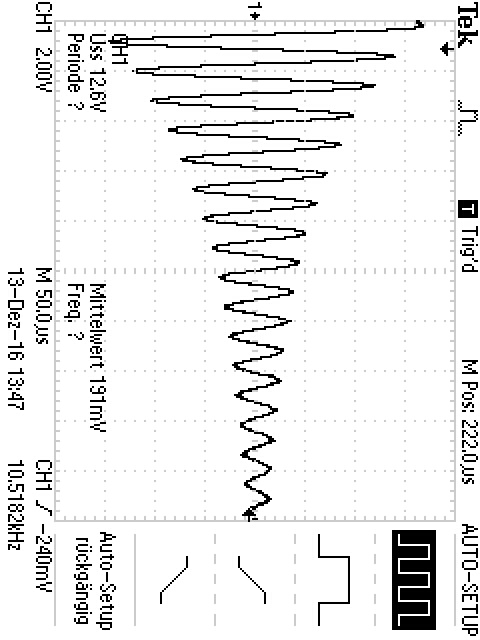
\includegraphics[width=0.52\textwidth,angle=90]{Bilder/a)correct/F0002TEK.JPG}
	\caption{Zeitlicher Verlauf der Spannungsamplitude am Kondensator nach Anregung durch einen Nadelimpuls.}
	\label{fig:spannungsamplitude}
\end{figure}
In Tabelle \ref{tab:messung1} befinden sich die gemessenen Daten der Spannungsamplituden $U_C$ und die zugehörigen Zeiten $t$.
Der Verlauf der Spannungsamplitude ist in Abbildung \ref{fig:spannungsamplitude} abgebildet. Die zugehörige Einhüllende ist in Abbildung \ref{fig:einhüllende} dargestellt.
Da sich $U_\text{0}$ nach dem Ohmschen Gesetz nur um einen Faktor von $I_\text{0}$ unterscheidet, ergibt sich nach Gleichung \eqref{eqn:schwingi} die Einhüllende mittels
\begin{equation}
	A=A_\text{0} \mathrm{e}^{-2 \pi \mu t} \text{.}
\end{equation}
Die Ausgleichsrechnung mittels Scipy und Python liefert die Werte:
\begin{equation*}
	A_0 =  (6.60 \pm 0.04) \,\si{\volt} \text{,}
\end{equation*}
\begin{equation*}
	\mu =  (851.8 \pm 7.5) \, \frac{1}{\si{\second}} \text{.}
\end{equation*}

$R_\text{eff}$ lässt sich nun mittels $\mu$ über Gleichung \eqref{eqn:defis} ermitteln. $T_\text{ex}$ ergibt sich nun nach Gleichung \eqref{eqn:abkling}.
Mittels Scipy und Python ergeben sich die Größen samt ihrer Fehler zu:
\begin{equation*}
	T_{\text{ex}}=(18.7 \pm 0.2) \cdot 10^{-5}\,\si{\second} \text{,}
\end{equation*}

\begin{equation*}
	R_{\text{eff}}= (108.2 \pm 1.0) \,\si{\ohm} \text{.}
\end{equation*}

Für die weiteren Berechnungen wird der Innenwiderstand des Generators nun mitbetrachtet.

%%%%%%%%%%%%%%%%%%%%%%%%%%%%%%%%%%%%%%%%%%%%%%%%%%%%%%%%%%%%%%%%%%%%%%%%%%%%%%%%%%%%%%%%%%5 <---die ist nice
\subsection{Bestimmung des Dämpfungswiderstandes $R_{\text{ap}}$}

Nach Gleichung \eqref{eqn:apigrenz} ergibt sich der Widerstand $R_{\text{ap}}$, bei dem der
aperiodische Grenzfall eintritt zu
\begin{equation}
	R_{\text{ap}} = \pm \sqrt{\frac{4L}{C}} \, \text{,}
	\label{eqn:rap}
\end{equation}
wobei der positive Wert -- also die physikalisch relevante Größe -- betrachtet wird.
Mit den notierten Werten und Gauß'scher Fehlerfortpflanzung erhält man schließlich
\begin{equation*}
	R_{\text{ap}} = (4390 \pm 9) \, \si{\ohm} \text{.}
\end{equation*}

Der gemessene Wert ist $R_{\text{ap}} = \SI{3400}{\ohm}$.
%%%%%%%%%%%%%%%%%%%%%%%%%%%%%%%%%%%%%%%%%%%%%%%%%%%%%%%%%%%%%%%%%%%%%%%%%%%%%%%%%%%%%%%%%%%%%%
\subsection{Frequenzabhängigkeit der Kondensatorspannung an einem Serienresonanzkreis}
Die gemessenen Daten zur Bestimmung der Resonanzüberhöhung und der Breite $ \omega_1 - \omega_2 $ der Resonanzkurve befinden sich in Tabelle \ref{tab:Kuh}.
In Abbildung \ref{fig:q} ist die normierte Kondensatorspannung $\frac{U_{\mathrm{C}}}{U_{\mathrm{0}}}$ gegen die Frequenz $\omega$ halblogarithmisch aufgetragen.

\begin{figure}
	\centering
	\includegraphics[width=0.9\textwidth]{build/c.pdf}
	\caption{Frequenzabhängigkeit der normierten Kondensatorspannung in halblogarithmischer Darstellung.}
	\label{fig:q}
\end{figure}
\begin{table}
	\caption{Messdaten zur Untersuchung der Frequenzabhängigkeit der Kondensatorspannung zur Bestimmung der Güte $q$ und Breite $\omega_+ - \omega_- $.}
	\label{tab:Kuh}
	\centering
	\begin{tabular}{ccc}
		\toprule
		$f$/$\cdot 10^{3} \si{\Hz}$ & $U_\text{C}$/$\si{\volt}$ & $\frac{U(t)}{U_\text{C}}$ \\
		\midrule
		1.0                         & 2.52                      & 0.93                      \\
		5.0                         & 3.40                      & 0.97                      \\
		10.0                        & 3.56                      & 1.02                      \\
		14.0                        & 3.88                      & 1.11                      \\
		17.0                        & 4.12                      & 1.18                      \\
		20.0                        & 4.68                      & 1.34                      \\
		22.0                        & 5.24                      & 1.50                      \\
		24.0                        & 5.92                      & 1.69                      \\
		26.0                        & 6.84                      & 1.95                      \\
		28.0                        & 8.40                      & 2.40                      \\
		29.0                        & 9.30                      & 2.66                      \\
		30.0                        & 10.10                     & 2.89                      \\
		31.0                        & 10.90                     & 3.21                      \\
		32.0                        & 11.70                     & 3.55                      \\
		34.0                        & 11.90                     & 3.61                      \\
		36.0                        & 10.50                     & 3.18                      \\
		38.0                        & 8.30                      & 2.52                      \\
		40.0                        & 6.50                      & 1.86                      \\
		45.0                        & 4.00                      & 1.14                      \\
		50.0                        & 2.80                      & 0.80                      \\
		75.0                        & 0.75                      & 0.23                      \\
		100.0                       & 0.35                      & 0.11                      \\
		\bottomrule
	\end{tabular}
\end{table}

Aus den Messdaten wird die Resonanzüberhöhung $q$ abgelesen zu
\begin{equation*}
	q_\mathrm{Experiment}= 3.61 \, .
\end{equation*}
Aus Formel \eqref{eqn:guete} ergibt sich $q$ zu
\begin{equation*}
	q_\mathrm{Theorie}= (3.923 \pm 0.009) .
\end{equation*}

\begin{figure}
	\includegraphics[width=0.9\textwidth]{build/breite.pdf}
	\caption{Linearer Plot der normierten Kondensatorspannung gegen die Frequenz zur Bestimmung der Güte und der Breite der Resonatorfrequenz.}
	\label{fig:breite}
\end{figure}
Zur Untersuchung der Breite der Resonanzkurve wird der Bereich um die Resonanzfrequenz
wie in Abbildung \ref{fig:breite} linear dargestellt.
Zusätzlich wird $\frac{q_\mathrm{Experiment}}{\sqrt{2}}$ eingezeichnet, sodass die Breite der Resonatorfrequenz abgelesen werden kann.
Aus der Abbildung wurde die Breite abgelesen zu:
\begin{equation*}
	\text{Abgelesen}: \omega_+ - \omega_- \approx 9.25 \cdot 10^{3} \,\si{\Hz} \text{,}
\end{equation*}
nach Formel \eqref{eqn:breite} ergibt sich:
\begin{equation*}
	\text{Theorie}: 	\omega_+ - \omega_- \approx \frac{R}{L}\cdot \frac{1}{2\pi}=(8.81\pm 0.03) \cdot 10^{3} \,\si{\Hz} \text{.}
\end{equation*}
%%%%%%%%%%%%%%%%%%%%%%%%%%%%%%%%%%%%%%%%%%%%%%%%%%%%%%%%%%%%%%%%%%%%%%%%%%%%%%%%%%%%%%%%%%%%%%
\subsection{Frequenzabhängigkeit der Phasenverschiebung}

Die Messwerte zur Untersuchung der Frequenzabhängigkeit der Phasenverschiebung zwischen Kondensator- und Erregerspannung sind in Tabelle \ref{tab:muh} aufgetragen.
In Abbildung \ref{fig:phasenplot} sind diese halblogarithmisch dargestellt.
Hier sei angemerkt, dass die Phasenverschiebung $\phi$ mittels $\phi = 2\pi \, \frac{a}{b}$ bestimmt wird, wobei $a$ der gemessenen Zeitdifferenz zwischen zwei Nulldurchgängen und $b$ der Periodendauer also $\frac{1}{\omega}$ entspricht.

\begin{table}
	\caption{Messdaten zur Untersuchung der Phasenverschiebung zwischen Kondensator- und Erregerspannung.}
	\centering
	\label{tab:muh}
	\begin{tabular}{cccc}
		\toprule
		$\omega$ / $\si{\Hz}$ & $a$ / $\si{\micro\second}$ & $b$ / $\si{\micro\second}$ & $\phi$ / $\si{\radian}$ \\
		\midrule
		1.0                   & 4.0                        & 1000.0                     & 0.02513                 \\
		5.0                   & 6.0                        & 200.0                      & 0.18850                 \\
		10.0                  & 3.4                        & 100.0                      & 0.21363                 \\
		14.0                  & 2.6                        & 71.4                       & 0.22871                 \\
		17.0                  & 2.4                        & 58,8                       & 0.25635                 \\
		20.0                  & 2.4                        & 50.0                       & 0.30159                 \\
		22.0                  & 2.6                        & 45.5                       & 0.35940                 \\
		24.0                  & 3.0                        & 41.7                       & 0.45239                 \\
		26.0                  & 3.2                        & 38.5                       & 0.52276                 \\
		28.0                  & 3.2                        & 35.7                       & 0.56297                 \\
		29.0                  & 3.2                        & 34.5                       & 0.58308                 \\
		30.0                  & 4.0                        & 33.3                       & 0.75398                 \\
		31.0                  & 4.6                        & 32.3                       & 0.89598                 \\
		32.0                  & 5.6                        & 31.3                       & 1.12595                 \\
		34.0                  & 7.8                        & 29.4                       & 1.66630                 \\
		36.0                  & 9.2                        & 27.8                       & 2.08099                 \\
		38.0                  & 10.0                       & 26.3                       & 2.38761                 \\
		40.0                  & 10.2                       & 25.0                       & 2.56354                 \\
		45.0                  & 10.2                       & 22.2                       & 2.88398                 \\
		50.0                  & 9.8                        & 20.0                       & 3.07876                 \\
		75.0                  & 6.7                        & 13.3                       & 3.15730                 \\
		100.0                 & 5.3                        & 10.0                       & 3.33009                 \\
		\bottomrule
	\end{tabular}
\end{table}



\begin{figure}
	\centering
	\includegraphics[width=0.9\textwidth]{build/taskd.pdf}
	\caption{Frequenzabhängigkeit der Phasenverschiebung zwischen Kondensator- und Erregerspannung halblogarithmisch aufgetragen.}
	\label{fig:phasenplot}
\end{figure}

Um die Resonatorfrequenz bzw. $\omega_1$ und $\omega_2$ besser ablesen zu können, wird der Bereich um die Resonatorfrequenz linear geplottet.
Der zugehörige Plot befindet sich in Abbildung \ref{fig:phasenplotlinear}.

Aus dem Plot werden die entsprechenden Werte abgelesen und die Theoriewerte werden nach Gleichung \eqref{eqn:omega12} bzw. \eqref{eqn:omega} bestimmt.
Die abgelesenen bzw. berechneten Werte sind in Tabelle \ref{tab:senseless_table} aufgetragen.
\begin{table}
	\caption{Experimentell und theoretisch bestimmte Werte für die Resonatorfrequenz und $\omega_{1,2}$.}
	\centering
	\label{tab:senseless_table}
	\begin{tabular}{cccc}
		\toprule
		                   & $\omega_1$ / $\si{\kilo\hertz}$ & $\omega_{\mathrm{res}}$ / $\si{\kilo\hertz}$ & $\omega_2$ / $\si{\kilo\hertz}$ \\
		\midrule
		\text{Abgelesen}   & 30.2                            & 33.7                                         & 37.7                            \\
		\text{Theoriewert} & 30.4 \pm 0.1                    & 34.0 \pm 0.1                                 & 39.2 \pm 0.1                    \\
		\bottomrule
	\end{tabular}
\end{table}
\begin{figure}
	\centering
	\includegraphics[width=0.9\textwidth]{build/taskdlinear.pdf}
	\caption{Frequenzabhängigkeit der Phasenverschiebung zwischen Kondensator- und Erregerspannung linear dargestellt.}
	\label{fig:phasenplotlinear}
\end{figure}
